In this chapter, we perform evaluation on our model and the other algorithms, the repository of our model is provided in github \footnote{\url{https://github.com/cwleung/LKJTM}}.
\section{Experiment Testing}
The experiment will be conducted with a number of existing proposed topic models as mentioned related work section above. We conduct the experiment with those baseline algorithms and evaluate them in terms of accuracy and running time. Some of the source code of competitive were provided by their authors in Github\footnote{For instance, Correlated Topic Model (CTM), \href{https://github.com/blei-lab/ctm-c}{https://github.com/blei-lab/ctm-c}}. The outcome result will be extensively studied and conclude the insight behind the algorithms and methodologies. Detail to be stated in section \ref{AD}.
\section{Algorithmic Settings}
% optimization algorithm
To perform posterior inference, we employed Stochastic Variational Inference (SVI) \cite{hoffman_stochastic_2013} for the optimization problem. We set the minibatch size to 1024 documents.
% Other model
For LDA, we applied the model provided from sklearn package (version 0.24.0) \footnote{Sklearn website \url{https://scikit-learn.org/stable/index.html}}. For ETM, we run the experiment with the parameter suggested \cite{dieng_topic_2019}. For ProdLDA, we perform optimization with inference network architecture as described in the paper \cite{srivastava_autoencoding_2017}. 
% learning rate
To perform optimization, we use Adam for the gradient ascent algorithm, and we set the learning rate to 1e-3.
% l2-regularization factor
we use $ \mathcal{l-2} $ regularization to the 
% inference network [size, activation function, dropout, batch-norm]
We use 
% Transformer settings

% 
\section{Dataset}To evaluate the performance of the model, we select the two most poplar data set in the context of topic model evaluation. 20Newsgroups and Reuter RCV1-v2 datasets. 20NewsGroup consist of 18,846 news group documents \footnote{\url{http://qwone.com/~jason/20Newsgroups/}} and the RCV1-v2 includes 10,000 documents in total. Both of the dataset will be preprocessed to remove stopwords and stemming before the evaluation. If desirable, it will also to be applied to NIST TREC dataset and NII NTCIR dateset for further application studies.
\section{Data Preprocessing}
We perform data preprocessing, tokenization, stopword removal, lemmatization, and set the 
\section{Models}
We compare the model performance with a numbers of rivals. We take Latent Dirichlet Allocation (LDA) as the baseline model.
\section{Quantitative Result}
In this section, we evaluate the model with the following metric adopted from \cite{dieng_dynamic_2019}: Perplexity, Topic Coherence (TC), Topic Diversity (TD). %and Topic Quality (TQ).\begin{center}
\paragraph{Perplexity}The proposed model will be evaluated with perplexity metric. The metric will examine how well the model can tackle with unseen data. It is equivalent algebraically to the inverse of the geometric mean per-word likelihood. Lower perplexity scores mean better.\begin{equation*}
\text{Perplexity}(D_{test})=\exp{{-\frac{\sum_{d=1}^{M}\sum_{m=1}^{N_d}\log p(w_{dm})}{\sum_{d=1}^{M}N_d}}}
\end{equation*}
\paragraph{Topic Coherence}Topic Coherence \cite{mimno_optimizing_2011}
\begin{equation*}
TC=\frac{1}{K}\sum_{k=1}^{K}\frac{1}{45}\sum_{i=1}^{10}\sum_{j=i+1}^{10}f(w_i^{(k)},w_j^{(k)})\end{equation*}
where $\{w_1^{(k)},\cdots,w_{10}^{(k)}\}$ denotes top-10 most likely words in topic k. And function $f(\cdot,\cdot)$ is te normalized pointwise mutual information.\begin{equation*}
f(w_i,w_j)=\frac{\log\frac{P(w_i,w_j)}{P(w_i)P(w_j)}}{-\log P(w_i,w_j)}\end{equation*}
\paragraph{Topic Diversity} In order to compare how the words each topic are differentiate the others. We applied the Topic Diversity metric \cite{dieng_topic_2019}. Topic Diversity (TD) to be the percentage of unique words in the top 25 words of all topics. Diversity close to 0 indicates redundant topics; diversity close to 1 indicates more varied topics. We define the overall metric for the quality of a model’s topics as the product of its topic diversity and topic coherence.
\begin{align*}
TD=\frac{|A\cap B|}{|A \cup B|}
\end{align*}
where $ A $ and $ B $ are top-k words from two topics. 
% \paragraph{Topic Quality}
\begin{table}[]
\centering
\begin{tabular}{llll}
\hline
Model      & TC     & Perplexity  \\ \hline
Transformer & -0.311 & - \\
LDA & 0.183 & 2425.9 \\
ProdLDA		&  0.107 & 5652.0\\
ETM	     	&  0.177 & \textbf{1919.3}\\
\textbf{Our model}  & \textbf{0.206} & 3444.1 \\ \hline
\end{tabular}
\caption{Result of our implementation(topic k=20)}
\end{table}
\begin{table}[]
\centering
\begin{tabular}{llll}
\hline
Model      & TC     & Perplexity  \\ \hline
Transformer & -0.251 & - \\
LDA & 0.155 & \textbf{2536.1} \\
ProdLDA		&  0.074 & 5654.1\\
ETM	     	&  0.145 & 2603.9\\
\textbf{Our model}  & \textbf{0.199} & 3705.0 \\ \hline
\end{tabular}
\caption{Result of our implementation(topic k=50)}
\end{table}
\section{Qualitative Result}The proposed model will be evaluated with a number of specifically selected topic and examined with their performance separately. The result will be exhaustively compared with other existing models.
\begin{table}[]
\centering
\begin{tabular}{llll}
\hline
ETM  \\ \hline
space, nasa, gov, mr, president, health, research, year, center\\
windows, file, window, program, files, server, version, dos, image\\
god, people, jesus, christian, israel, bible, jews, christians, israeli\\
key, encryption, chip, clipper, keys, privacy, security, technology, government\\
gun, people, government, law, state, guns, article, weapons, control
\\ \hline
ETM  \\ \hline
space, nasa, gov, mr, president, health, research, year, center\\
windows, file, window, program, files, server, version, dos, image\\
god, people, jesus, christian, israel, bible, jews, christians, israeli\\
key, encryption, chip, clipper, keys, privacy, security, technology, government\\
gun, people, government, law, state, guns, article, weapons, control
\\ \hline
ETM  \\ \hline
space, nasa, gov, mr, president, health, research, year, center\\
windows, file, window, program, files, server, version, dos, image\\
god, people, jesus, christian, israel, bible, jews, christians, israeli\\
key, encryption, chip, clipper, keys, privacy, security, technology, government\\
gun, people, government, law, state, guns, article, weapons, control
\\ \hline
ETM  \\ \hline
space, nasa, gov, mr, president, health, research, year, center\\
windows, file, window, program, files, server, version, dos, image\\
god, people, jesus, christian, israel, bible, jews, christians, israeli\\
key, encryption, chip, clipper, keys, privacy, security, technology, government\\
gun, people, government, law, state, guns, article, weapons, control
\\ \hline
ETM  \\ \hline
space, nasa, gov, mr, president, health, research, year, center\\
windows, file, window, program, files, server, version, dos, image\\
god, people, jesus, christian, israel, bible, jews, christians, israeli\\
key, encryption, chip, clipper, keys, privacy, security, technology, government\\
gun, people, government, law, state, guns, article, weapons, control
\\ \hline
\end{tabular}
\caption{Testing}
\end{table}
\subsection{Visualization}
To clearly demonstrate the representation for , we applied t-SNE to map the topic-word representation into 2-dimension continuous space. In figure \ref{fig:tsne50t25w0}, .
%\begin{figure}
%\centering
%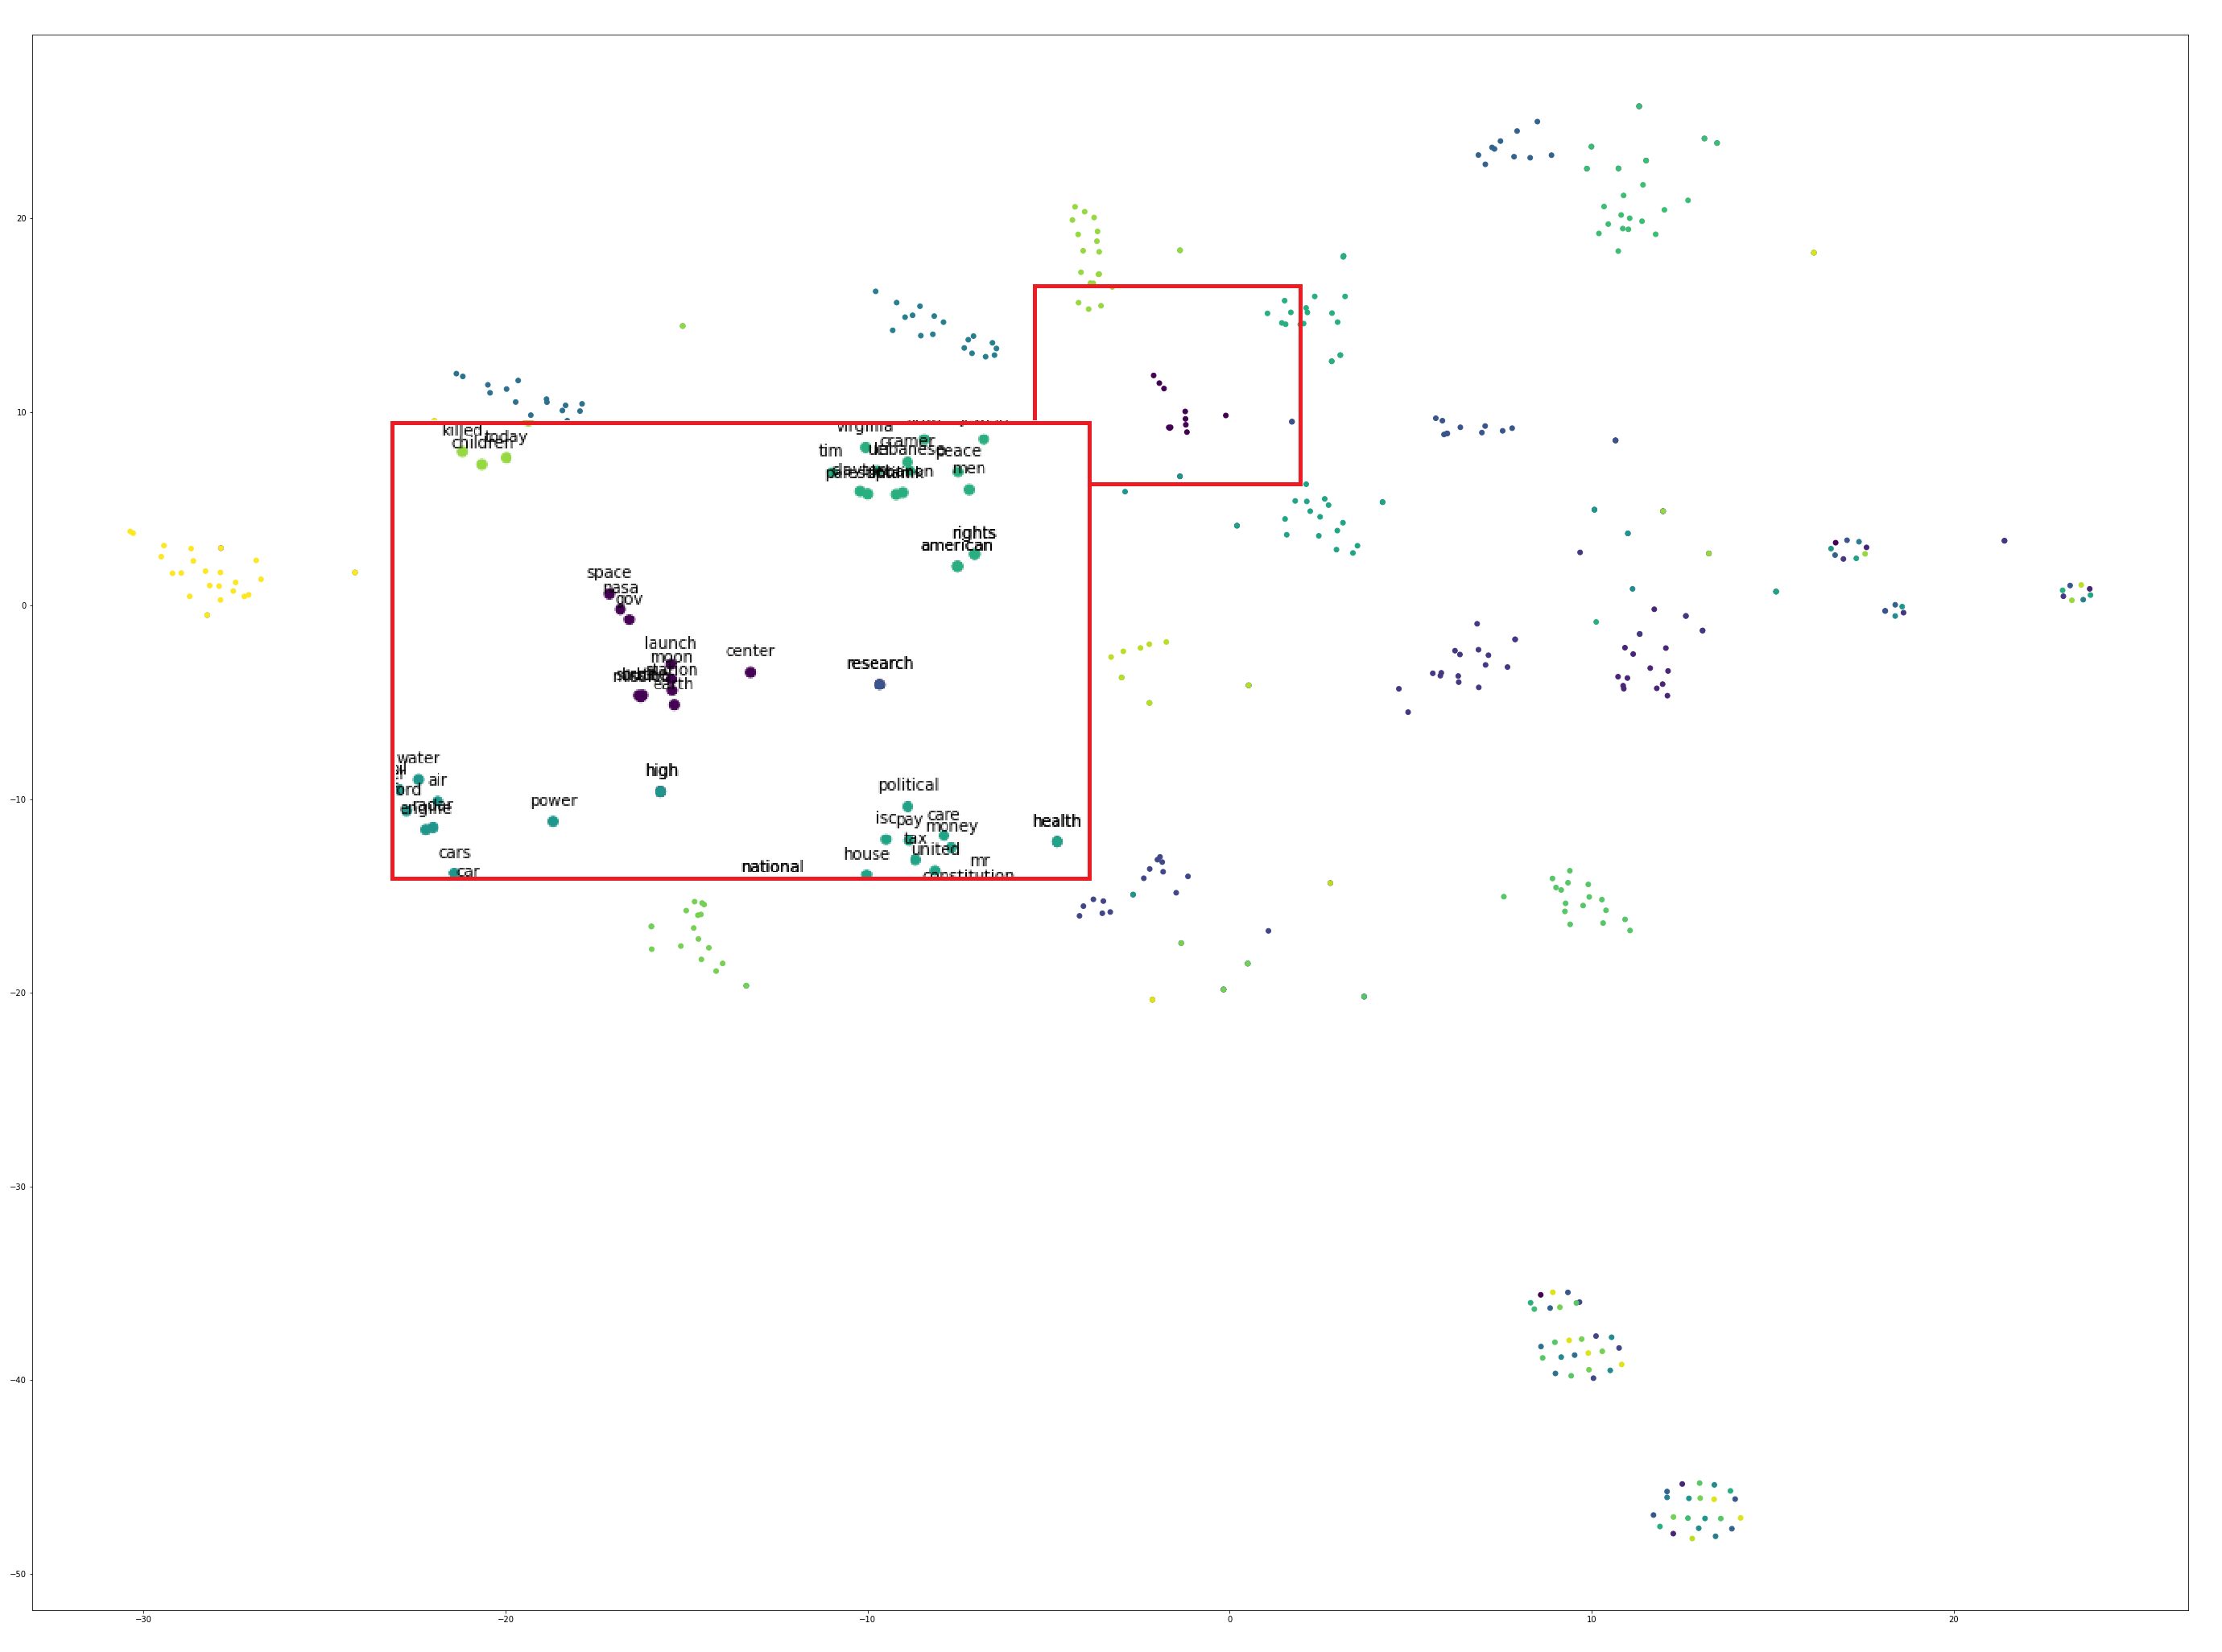
\includegraphics[width=1\linewidth]{figure/tsne_20t_25w_2}
%\caption{Visualization \#Topics:20}
%\label{fig:tsne20t25w2}
%\end{figure}
%\begin{figure}
%\centering
%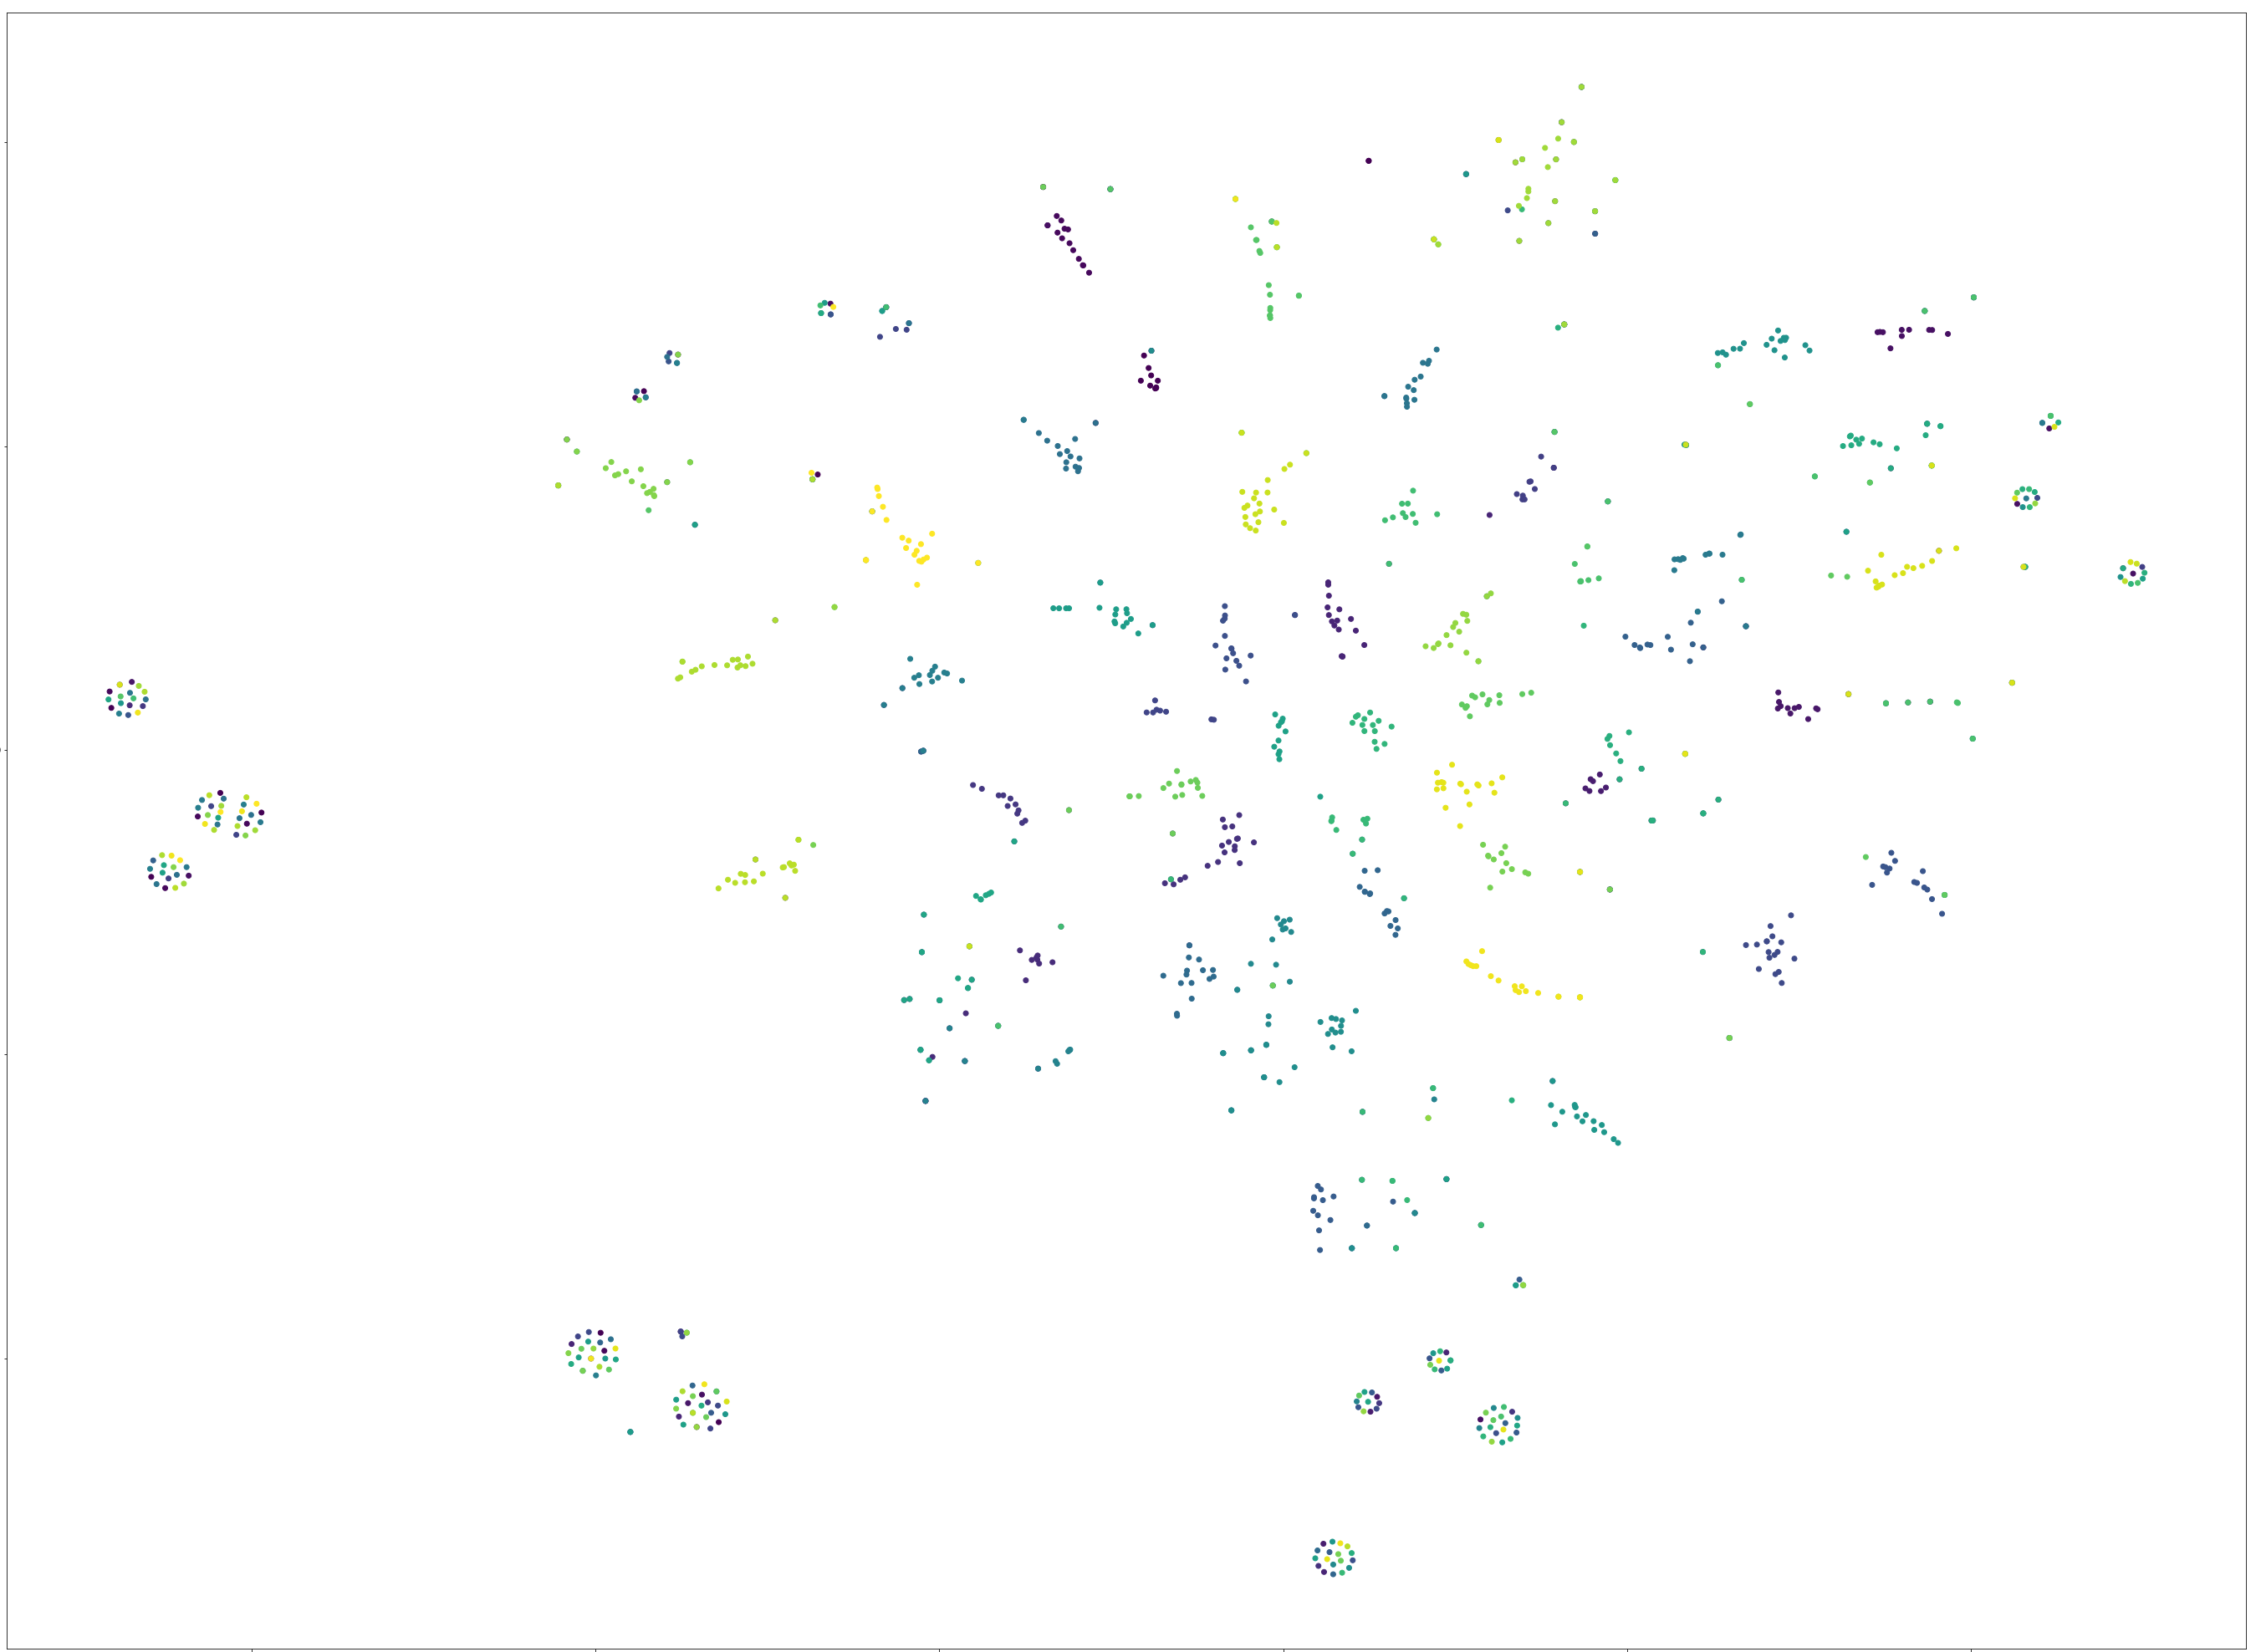
\includegraphics[width=1\linewidth]{figure/tsne_50t_25w_0}
%\caption{Visualization \#Topics:50}
%\label{fig:tsne50t25w0}
%\end{figure}
